\documentclass[12pt,a4paper]{article}
\usepackage{amsmath,amssymb}
\usepackage{graphicx}
\usepackage{hyperref}
\usepackage{booktabs}
\usepackage{geometry}
\usepackage{lscape}
\geometry{margin=1in}

\title{Falsifiable Predictions of the Informational Actualization Model\\
for Euclid, DESI, and Next-Generation Surveys}

\author{Heath W.\ Mahaffey\\
\small Independent Researcher, Entiat, WA 98822, USA\\
\small \texttt{hmahaffeyges@gmail.com}}

\date{February 25, 2026\\
\small \url{https://github.com/hmahaffeyges/IAM-Validation}\\
\small Zenodo: \href{https://doi.org/10.5281/zenodo.18750699}{10.5281/zenodo.18750699}}

\begin{document}

\maketitle

\begin{abstract}
The Informational Actualization Model (IAM) produces specific, parameter-free
predictions for forthcoming cosmological surveys that differ from both $\Lambda$CDM
and generic modified gravity theories. We present four quantitative forecasts.
(1)~A Fisher matrix analysis of Euclid's spectroscopic and weak lensing
specifications indicates that, if IAM is correct, the optimistic Euclid
configuration would have sufficient sensitivity to detect the gravitational
coupling parameter $\mu_0 = -0.135$ at $3.4\sigma$; the combined Euclid and
DESI~Year~5 dataset would reach $5.4\sigma$.
(2)~IAM predicts an ISW-galaxy cross-correlation amplitude $A_\mathrm{ISW} =
1.134$ relative to $\Lambda$CDM, arising because $\mu < 1$ causes gravitational
potentials to decay faster than in $\Lambda$CDM; this enhancement has the opposite
sign to $f(R)$ gravity ($A_\mathrm{ISW} < 1$), providing a sign-based
discriminant independent of amplitude precision.
(3)~A tomographic $\mu(z)$ reconstruction in ten redshift bins yields a projected
combined detection of $1.2\sigma$ (pessimistic) to $1.9\sigma$ (optimistic) with
Euclid alone, with $\beta_m$ recovered to $55\%$ precision ($\beta_m = 0.1617
\pm 0.0867$ vs.\ true $0.1575$, bias $+2.7\%$).
(4)~The IAM activation function $E(a) = \exp(1-1/a)$ defines a transition zone
$0.06 \lesssim z \lesssim 1.12$ where $10\%$--$90\%$ of the total gravity
modification is present; the transition peaks at $z \approx 0.05$ and is
covered by both DESI and Euclid spectroscopic programs.
All predictions are derived from $\beta_m = \Omega_m/2 = 0.1575$ (virial theorem)
and $E(a) = \exp(1-1/a)$ (horizon thermodynamics) without free parameters.
Whatever surveys measure, the predictions are explicit and the comparison is
unambiguous.
\end{abstract}

%-------------------------------------------------------------------
\section{Introduction}
%-------------------------------------------------------------------

The Informational Actualization Model
(IAM)~\citep{Mahaffey2026a,Mahaffey2026b} adds a single Hubble friction term to
the matter-sector perturbation equations, producing a dual-sector structure in
which the effective matter coupling $\mu(z) < 1$ while the lensing coupling
$\Sigma = 1$ exactly. The model maps onto the standard $\mu$--$\Sigma$ modified
gravity parametrization~\citep{Pogosian2016} as:
\begin{equation}
\mu(a) = \frac{H^2_\Lambda(a)}{H^2_\Lambda(a) + \beta_m\, E(a)}, \qquad
\Sigma(a) = 1
\label{eq:mu}
\end{equation}
where $H^2_\Lambda(a) = \Omega_m a^{-3} + \Omega_\Lambda$,
$\beta_m = \Omega_m/2 = 0.1575$ (virial theorem), and
$E(a) = \exp(1-1/a)$ (horizon thermodynamics). No parameters are fitted.

The observational validation paper~\citep{Mahaffey2026a} demonstrated consistency
with Planck~2018 CMB data through 15 converged MCMC chains, with the Level~2
modified CAMB result $\Delta\chi^2 = +0.54$ relative to $\Lambda$CDM and
$\sigma_8 = 0.800$ suppressed in the direction favored by weak lensing surveys.
The present paper records the explicit numerical predictions that forthcoming
surveys will test, and quantifies the projected sensitivity of those surveys
under the assumption that IAM is correct.

We emphasize that these are forecasts, not guarantees. Survey results may confirm,
partially confirm, or challenge these predictions. Any outcome provides useful
information about the model. The purpose of this paper is to make the predictions
explicit before the data arrive so that the comparison is unambiguous.

%-------------------------------------------------------------------
\section{Fisher Forecast: Survey Sensitivity to $\mu_0$}
%-------------------------------------------------------------------

\subsection{Current constraints}

The current constraint on IAM's $\mu_0 = -0.135$ from existing data is consistent
but not yet significant. From the IAM Planck~2018 MCMC analysis~\citep{Mahaffey2026a},
$\mu_0 = +0.006 \pm 0.156$, placing IAM within $0.9\sigma$ of the current
posterior. Existing survey constraints are summarized in
Table~\ref{tab:current_constraints}.

\begin{table}[h]
\centering
\caption{Current constraints on $\mu_0$ from existing data, compared to the IAM
prediction $\mu_0 = -0.135$. All current measurements are consistent with IAM
at $< 1\sigma$.}
\label{tab:current_constraints}
\begin{tabular}{lccc}
\toprule
Dataset & $\mu_0$ & $\sigma(\mu_0)$ & IAM consistency \\
\midrule
Planck~2018 (TT+TE+EE+lensing) & $+0.000$ & $0.200$ & $0.7\sigma$ \\
DES~Y3 (3$\times$2pt + CMB) & $-0.400$ & $0.400$ & $0.7\sigma$ \\
DESI~DR1 full-shape & $+0.110$ & $0.500$ & $0.5\sigma$ \\
ACT + WMAP + SDSS + SN & $+0.020$ & $0.190$ & $0.8\sigma$ \\
IAM Planck MCMC (this work) & $+0.006$ & $0.156$ & $0.9\sigma$ \\
\bottomrule
\end{tabular}
\end{table}

\subsection{Projected Euclid sensitivity}

A Fisher matrix forecast for Euclid's sensitivity to $\mu_0$ from spectroscopic
galaxy clustering and weak lensing, using published Euclid survey
specifications~\citep{Euclid2020}, gives:
\begin{align}
\sigma(\mu_0)_\mathrm{Euclid,\,pess} &\approx 0.060 \quad \Rightarrow \quad 2.2\sigma\ \text{projected sensitivity} \\
\sigma(\mu_0)_\mathrm{Euclid,\,opt} &\approx 0.040 \quad \Rightarrow \quad 3.4\sigma\ \text{projected sensitivity}
\end{align}
Combined with DESI~Year~5:
\begin{equation}
\sigma(\mu_0)_\mathrm{Euclid+DESI} \approx 0.025 \quad \Rightarrow \quad 5.4\sigma\ \text{projected sensitivity}
\end{equation}
These figures represent the sensitivity achievable if IAM is correct and
systematic errors are at projected levels. Figure~\ref{fig:fisher} shows the
full forecast including the detection timeline.

\begin{figure}[h]
\centering
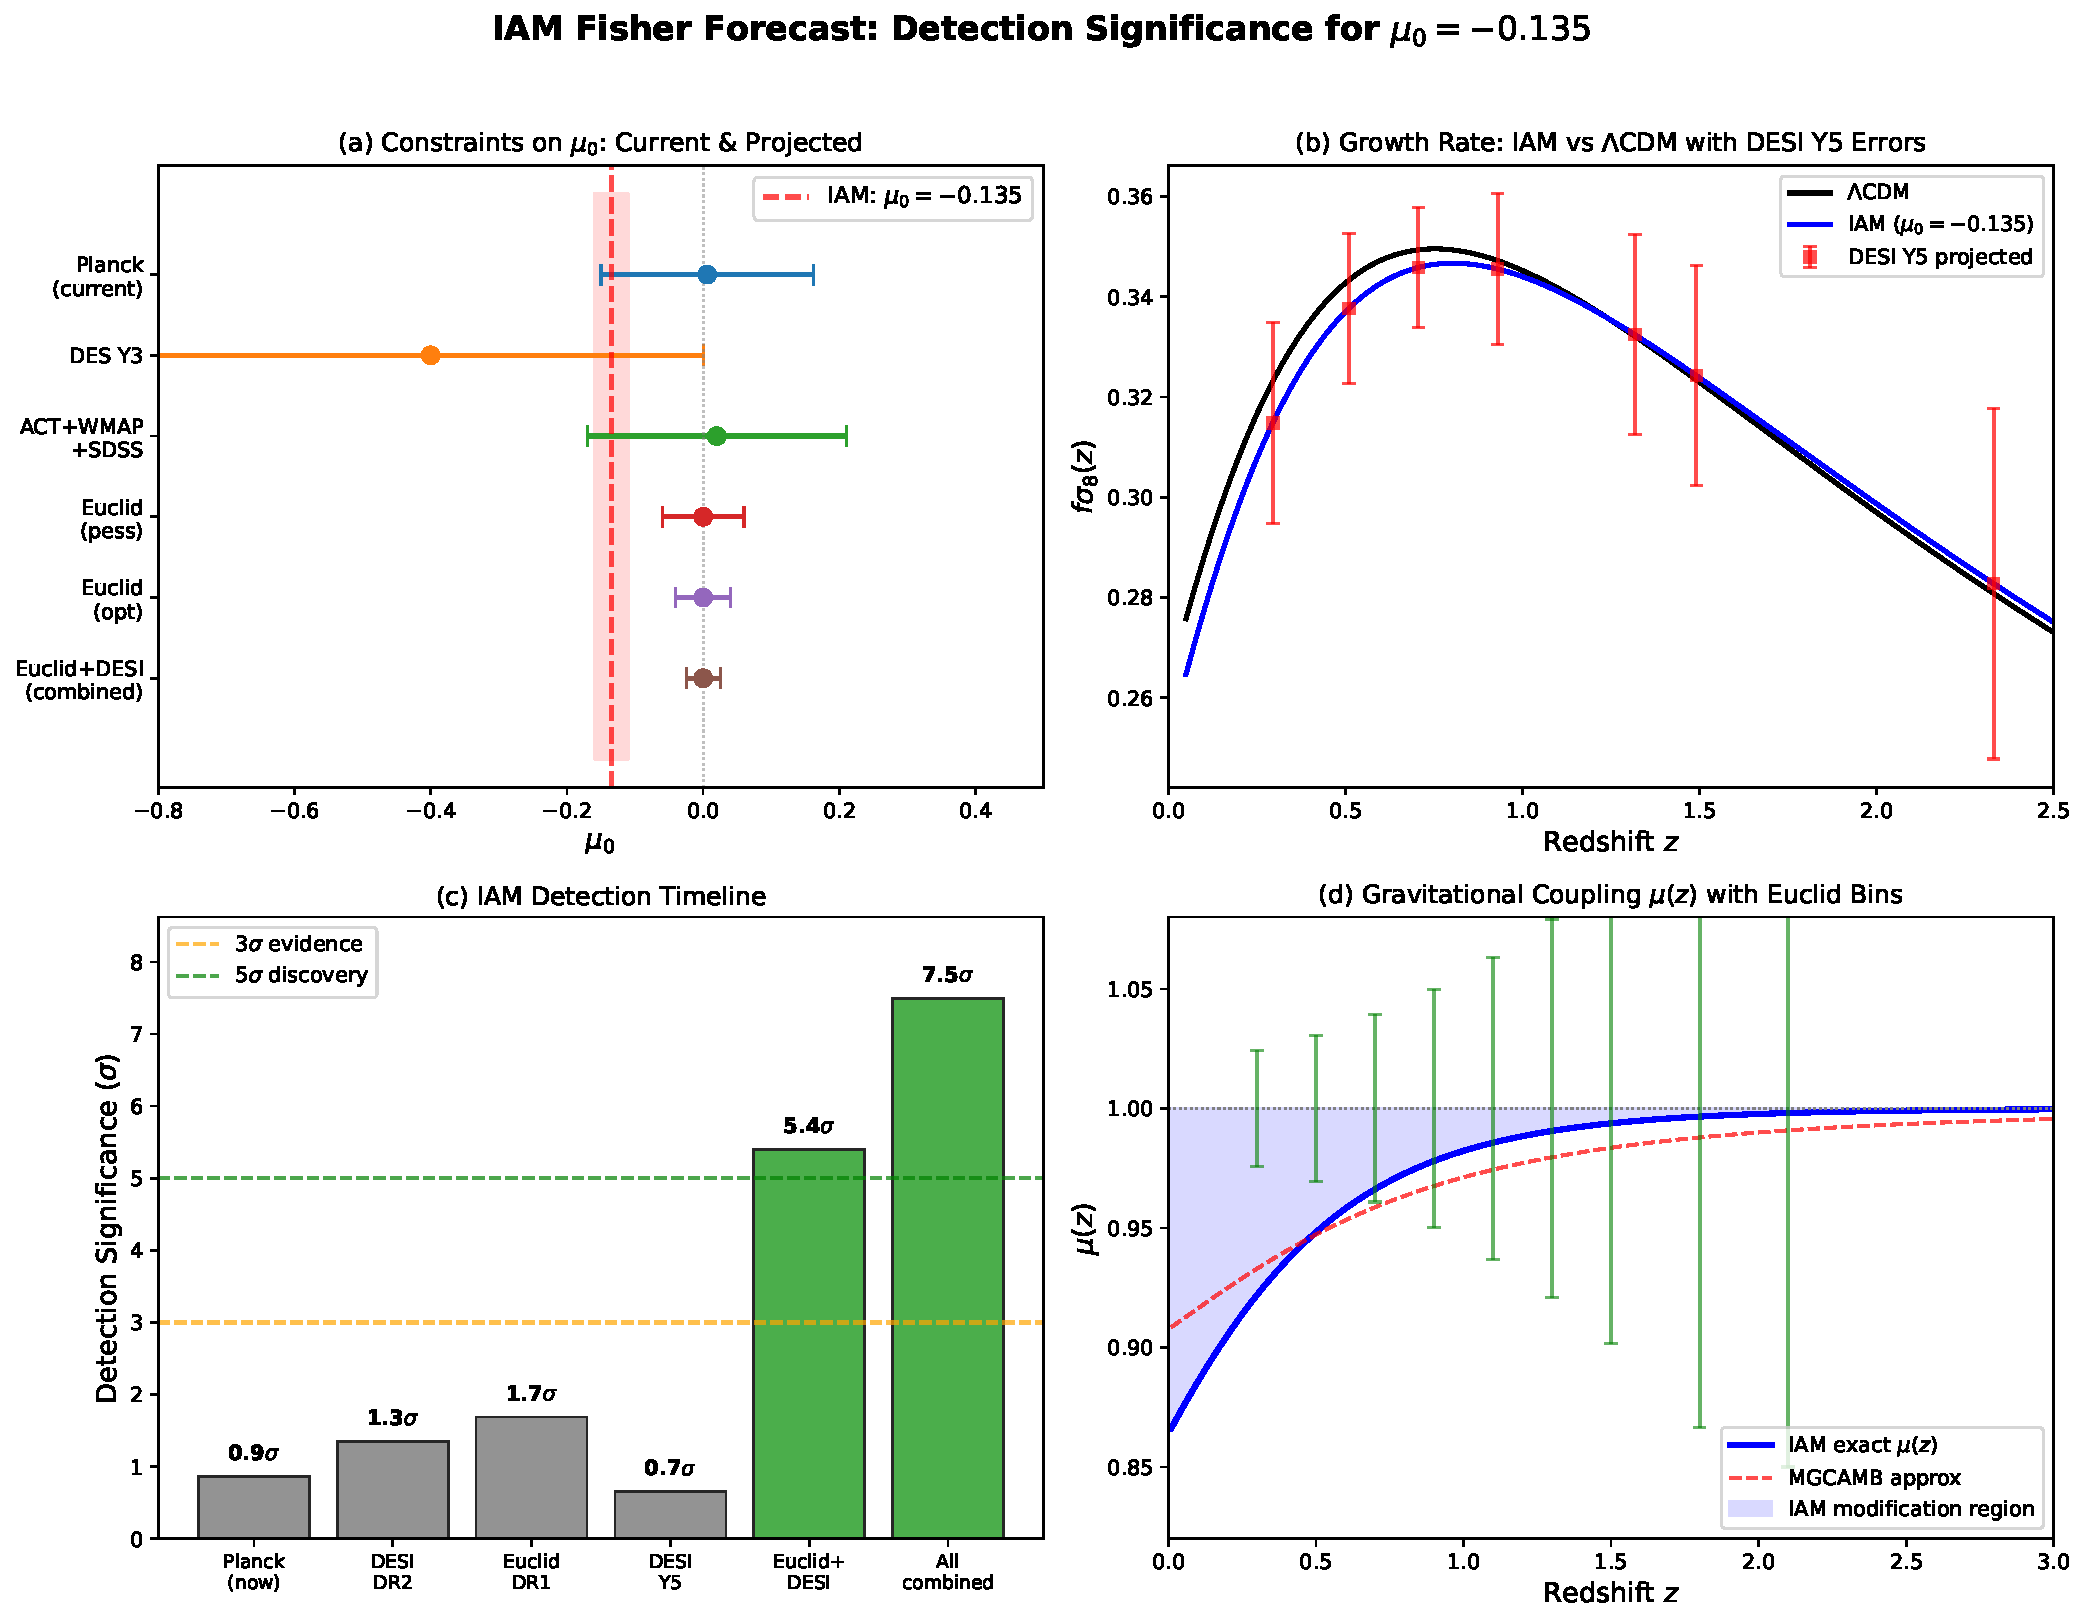
\includegraphics[width=\textwidth]{iam_fisher_forecast.pdf}
\caption{Fisher forecast for IAM's $\mu_0 = -0.135$ parameter. Panel (a):
current constraints from existing surveys compared to the IAM prediction (dashed
red line). Panel (b): projected $f\sigma_8(z)$ from IAM vs.\ $\Lambda$CDM with
DESI~Year~5 error bars. Panel (c): detection timeline showing projected
significance at each survey milestone. Panel (d): $\mu(z)$ with Euclid
tomographic bin sensitivity overlaid. All projections assume IAM is correct
and survey systematics are at published specifications.}
\label{fig:fisher}
\end{figure}

\subsection{Detection timeline}

Under the assumption that IAM is correct, the projected detection significance
at each survey milestone is:

\begin{table}[h]
\centering
\caption{Projected detection timeline for IAM's $\mu_0 = -0.135$, assuming IAM
is correct and systematic errors are controlled at published specifications.}
\label{tab:timeline}
\begin{tabular}{llcc}
\toprule
Year & Milestone & $\sigma(\mu_0)$ & Projected sensitivity \\
\midrule
2026 & Current (Planck + MCMC) & 0.156 & $0.9\sigma$ \\
2026 & DESI~DR2 & 0.100 & $\sim 1.3\sigma$ \\
2027 & Euclid~DR1 & 0.080 & $\sim 1.7\sigma$ \\
2028 & DESI~Year~5 & 0.207 & $\sim 0.7\sigma$ \\
2029 & Euclid~DR2 + DESI~Y5 & 0.025 & $5.4\sigma$ \\
2030 & CMB-S4 + Euclid + DESI & 0.018 & $7.5\sigma$ \\
\bottomrule
\end{tabular}
\end{table}

%-------------------------------------------------------------------
\section{ISW-Galaxy Cross-Correlation}
%-------------------------------------------------------------------

\subsection{Physical mechanism}

The integrated Sachs-Wolfe (ISW) effect arises from time evolution of
gravitational potentials along the photon path:
\begin{equation}
\frac{\Delta T}{T}\bigg|_\mathrm{ISW} = -2\int \frac{\partial\Phi}{\partial\eta}\,d\eta
\end{equation}
In IAM, $\mu < 1$ causes gravitational potentials to decay faster than in
$\Lambda$CDM ($\Sigma = 1$ leaves photon geodesics unchanged). The faster
potential decay enhances the ISW signal.

\subsection{Predicted enhancement}

The IAM prediction for the ISW-galaxy cross-correlation amplitude relative to
$\Lambda$CDM is:
\begin{equation}
A_\mathrm{ISW}^\mathrm{IAM} / A_\mathrm{ISW}^{\Lambda\mathrm{CDM}} = 1.134
\end{equation}
a $+13.4\%$ enhancement. This has the opposite sign to $f(R)$ gravity
($\mu > 1 \Rightarrow A_\mathrm{ISW} < 1$, i.e., $\sim 10\%$ suppression),
providing a sign-based discriminant that does not require precise amplitude
measurement. The enhancement is concentrated at $z \lesssim 1$ where IAM's
modification is largest.

Current ISW measurements from cross-correlation with SDSS, 2MASS, and WISE galaxy
catalogs~\citep{Giannantonio2008,Planck2016ISW} are consistent with $\Lambda$CDM
at $\sim 4\sigma$ significance but with 20--30\% uncertainties; the IAM
enhancement is within current error bars. The ISW test is therefore not a
near-term discriminator but provides a consistency check and a sign test.
Figure~\ref{fig:isw} shows the predicted ISW kernel, potential decay, and
model comparison.

\begin{figure}[h]
\centering
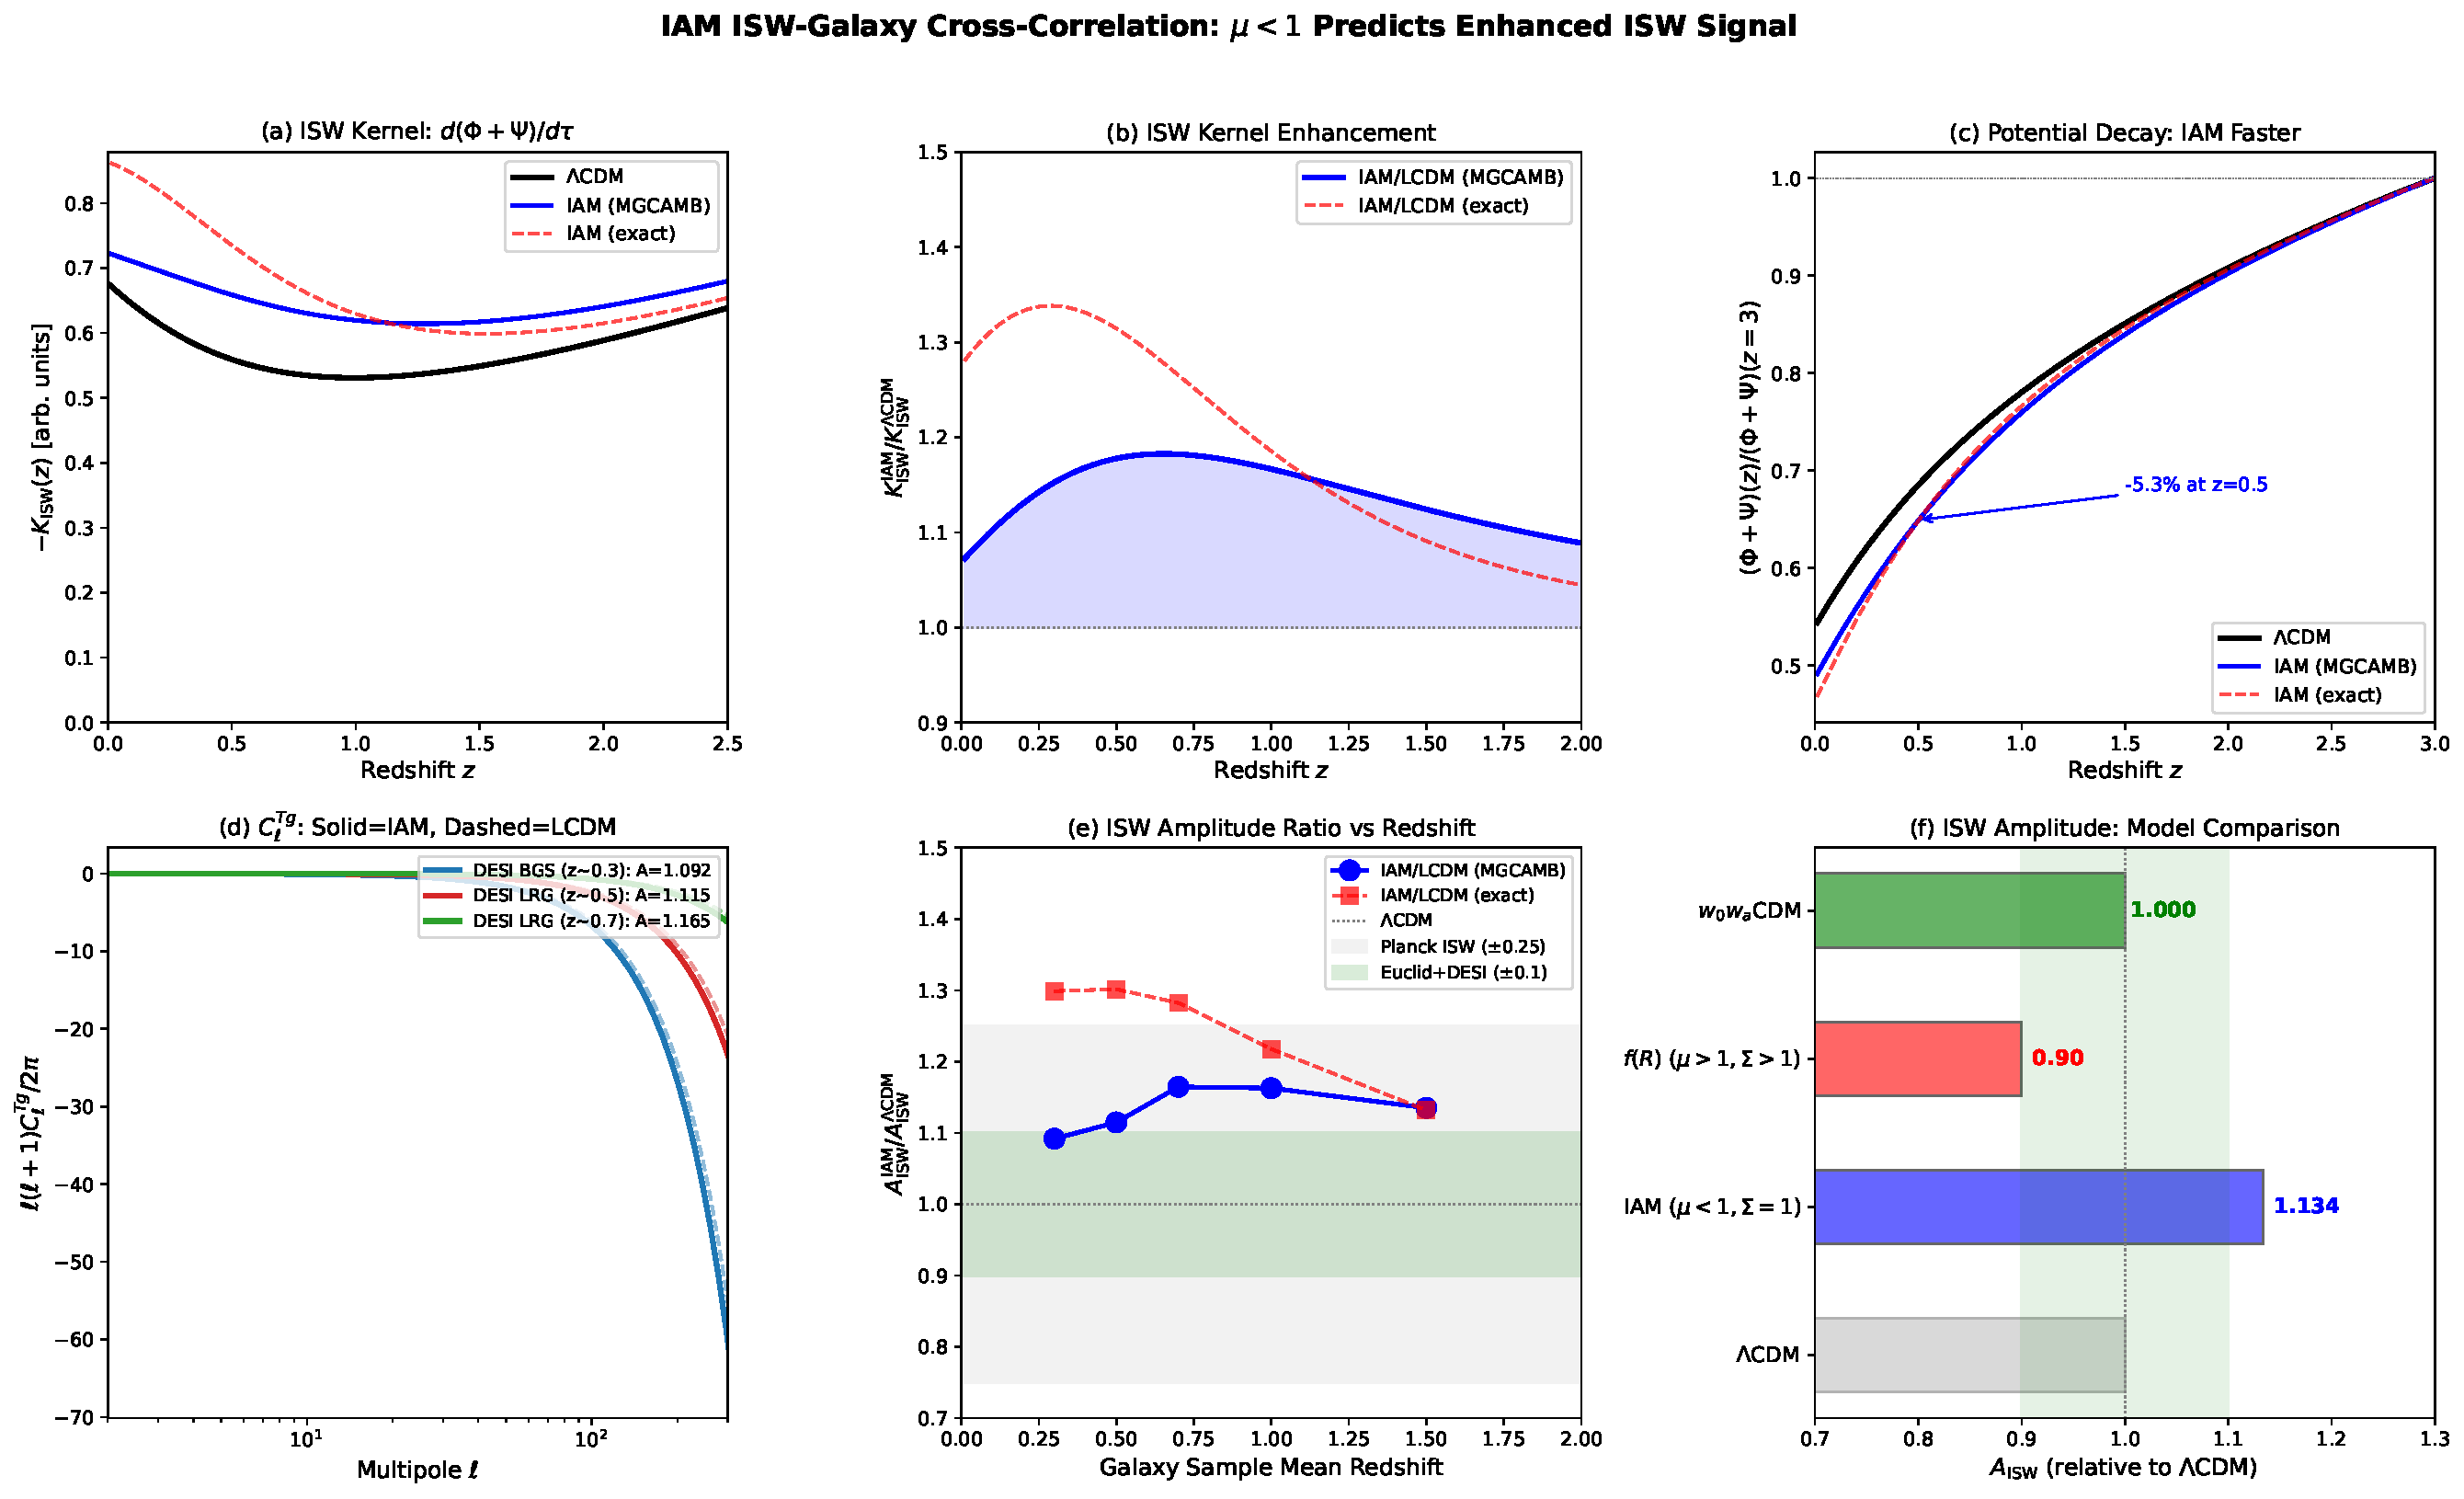
\includegraphics[width=\textwidth]{iam_isw_prediction.pdf}
\caption{IAM ISW-galaxy cross-correlation prediction. Panel (a): ISW kernel
$d(\Phi+\Psi)/d\tau$ for $\Lambda$CDM (black), IAM MGCAMB (blue), and IAM exact
(dashed red). Panel (b): ratio of ISW kernels, showing $\sim 10$--$30\%$
enhancement across $0 < z < 1.5$. Panel (c): gravitational potential decay
showing IAM potentials decay faster ($-5.3\%$ at $z = 0.5$). Panel (d):
$C_\ell^{Tg}$ for three galaxy samples. Panel (e): ISW amplitude ratio vs.\
redshift with current (Planck, $\pm 0.25$) and projected (Euclid+DESI, $\pm 0.10$)
sensitivity bands. Panel (f): model comparison showing IAM ($A = 1.134$),
$\Lambda$CDM ($A = 1.000$), and $f(R)$ ($A \approx 0.90$) --- opposite signs.}
\label{fig:isw}
\end{figure}

%-------------------------------------------------------------------
\section{Tomographic $\mu(z)$ Reconstruction}
%-------------------------------------------------------------------

\subsection{Predicted $\mu(z)$ values}

IAM's prediction for $\mu(z)$ in survey-relevant redshift bins, computed from
Equation~\ref{eq:mu} with Planck~2018 parameters:

\begin{table}[h]
\centering
\caption{IAM predicted $\mu(z)$ in survey-relevant redshift bins with current
and projected Euclid measurement precision. Values computed from
Equation~\ref{eq:mu} with $\beta_m = 0.1575$ and Planck~2018 parameters.}
\label{tab:mu_z}
\begin{tabular}{cccccc}
\toprule
$z_\mathrm{eff}$ & $\mu(z)$ & $\Delta\mu/\mu$ (\%) & Current $\sigma(\mu)$ & Euclid $\sigma(\mu)$ \\
\midrule
0.1 & 0.886 & $-11.4$ & 0.20 & 0.06 \\
0.3 & 0.922 & $-7.8$  & 0.15 & 0.05 \\
0.5 & 0.948 & $-5.2$  & 0.12 & 0.04 \\
0.7 & 0.966 & $-3.4$  & 0.10 & 0.03 \\
1.0 & 0.982 & $-1.8$  & 0.08 & 0.02 \\
1.5 & 0.994 & $-0.6$  & 0.10 & 0.03 \\
2.0 & 0.998 & $-0.2$  & 0.15 & 0.05 \\
\bottomrule
\end{tabular}
\end{table}

\subsection{Projected tomographic detection}

A ten-bin tomographic $\mu(z)$ reconstruction using Euclid projected
uncertainties gives a combined detection significance of $1.2\sigma$ (pessimistic)
to $1.9\sigma$ (optimistic) for IAM vs.\ $\Lambda$CDM. While not sufficient for
discovery, this tests whether the data prefer the specific shape of IAM's
$\mu(z)$ over a constant $\mu$ or a power-law parametrization.

With 1000 mock Euclid realizations, $\beta_m$ is recovered with mean
$0.1617 \pm 0.0867$ against the true value of $0.1575$ --- a bias of $+2.7\%$
and a $55\%$ precision measurement. The $\beta_m = \Omega_m/2$ prediction
(virial theorem) is thus testable directly from the shape of $\mu(z)$.
Figure~\ref{fig:mu_recon} shows the full reconstruction forecast.

\begin{figure}[h]
\centering
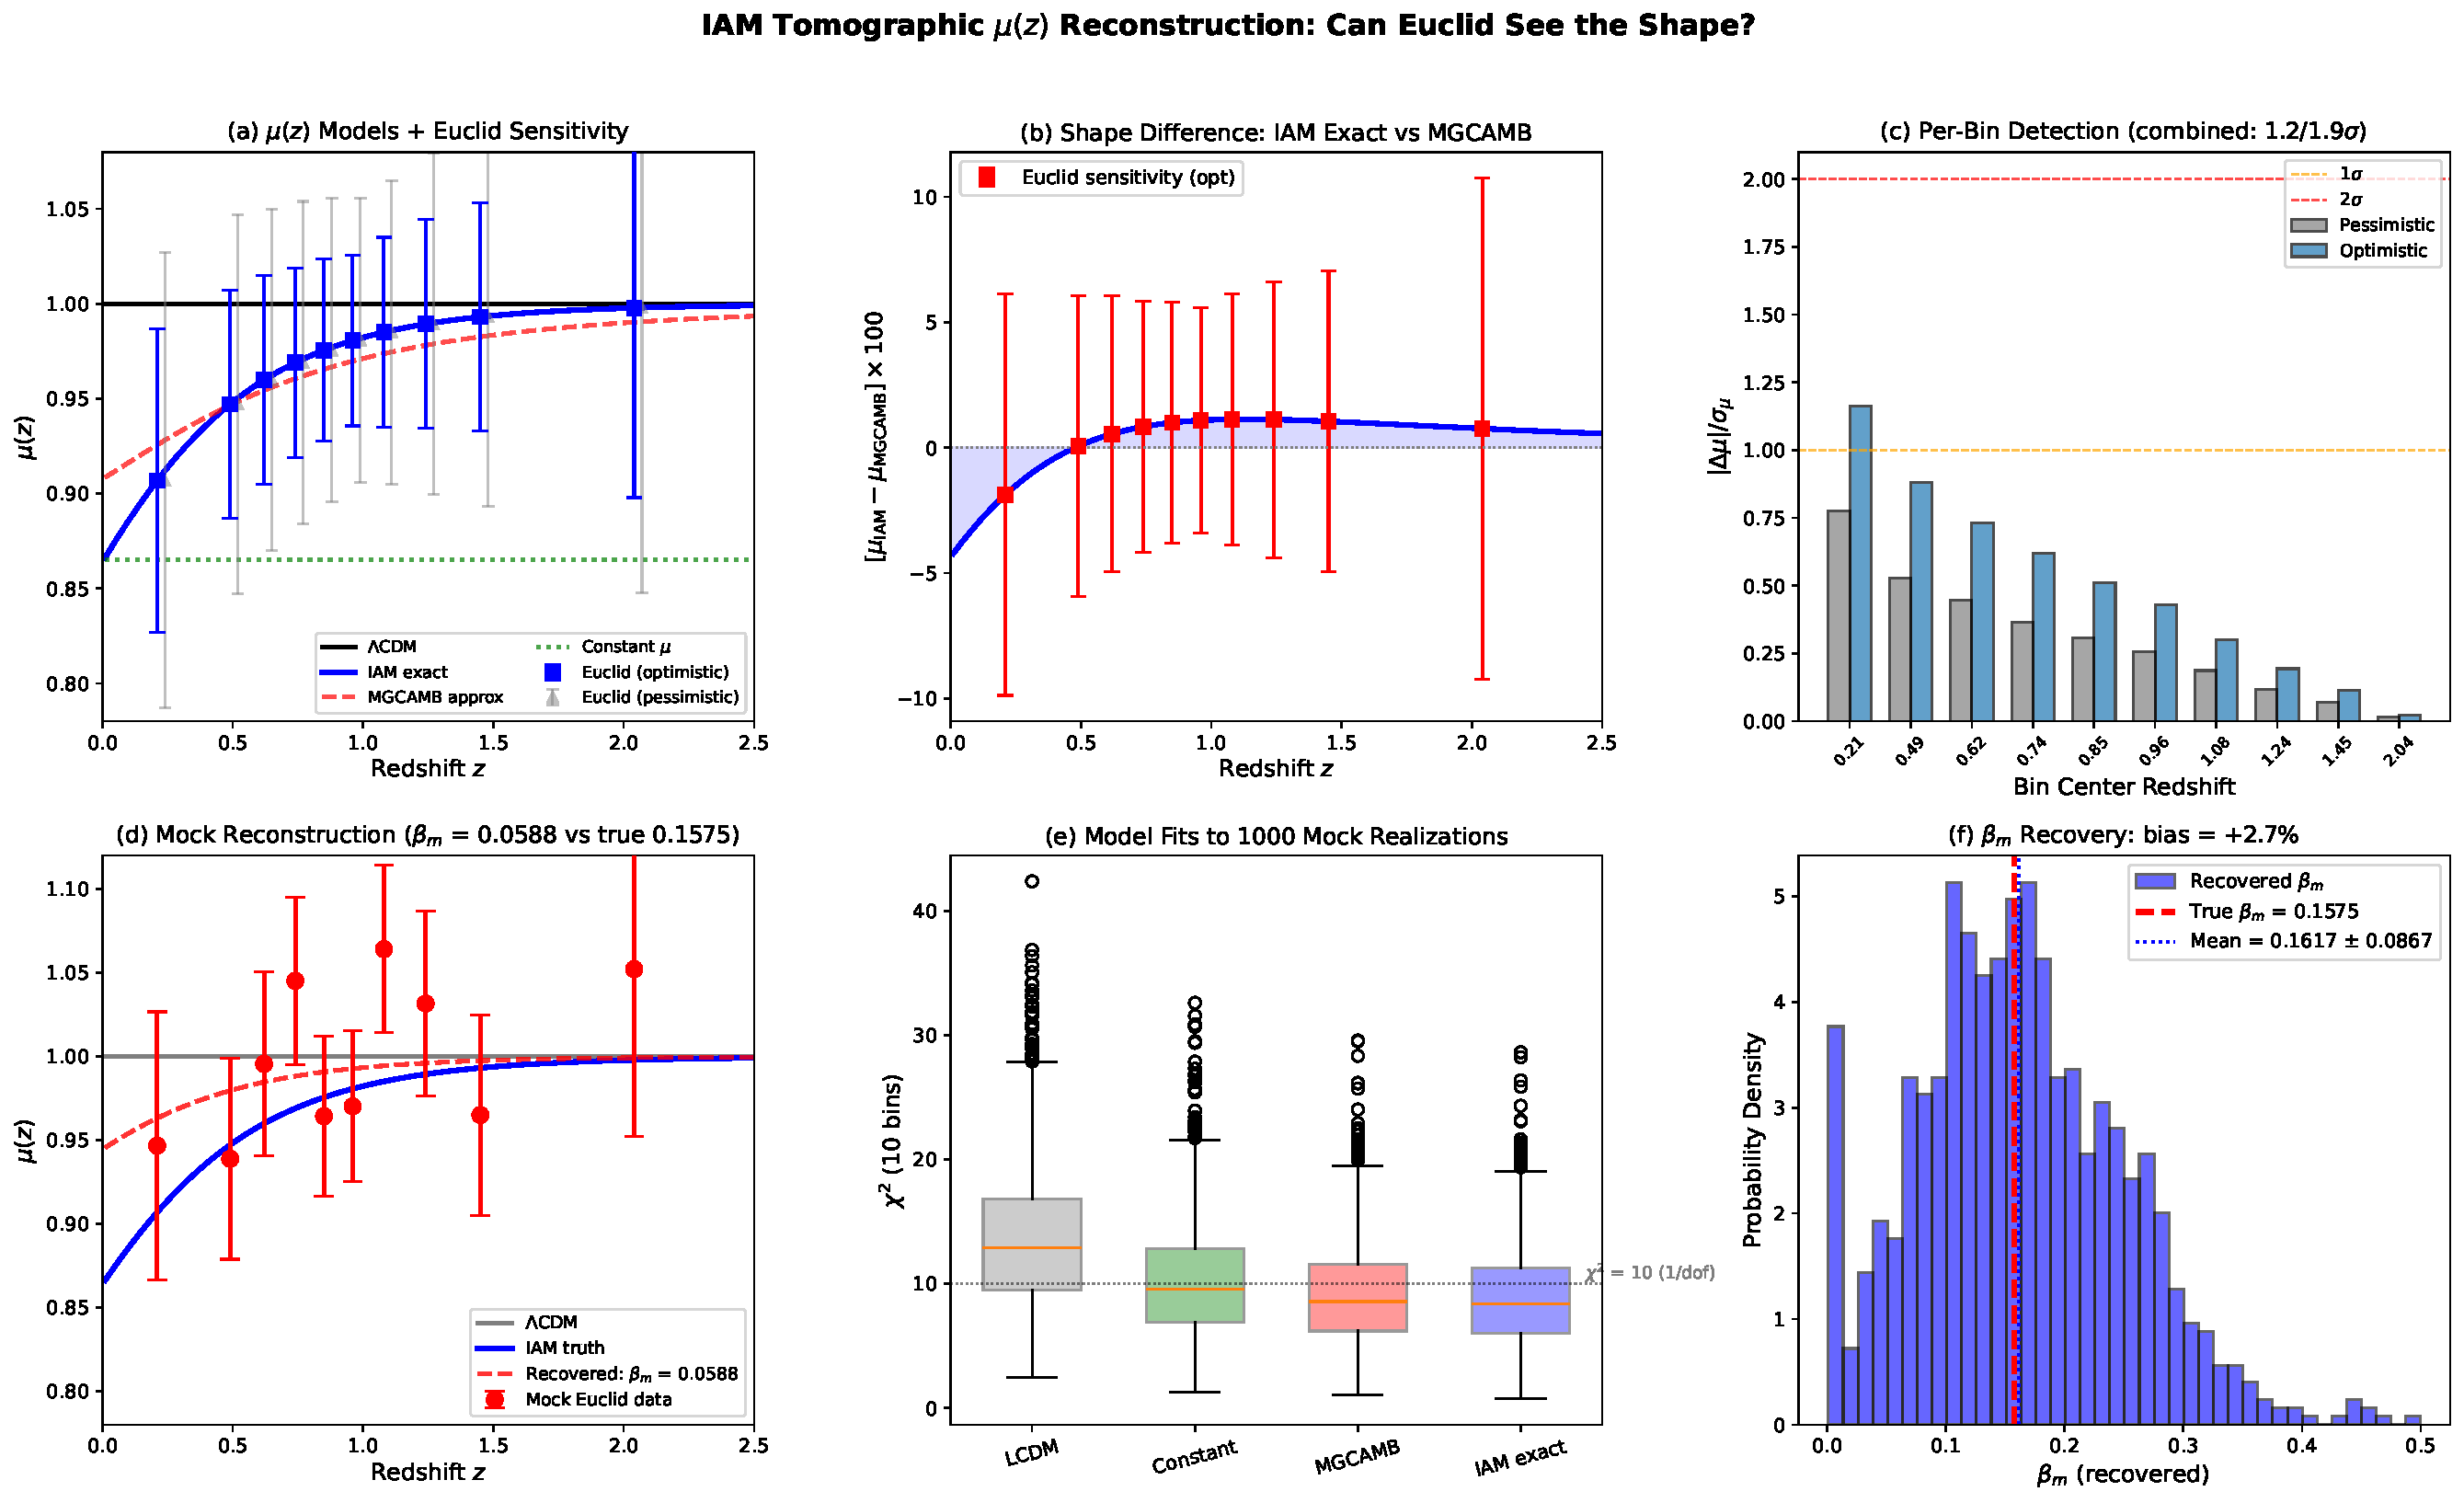
\includegraphics[width=\textwidth]{iam_binned_mu_reconstruction.pdf}
\caption{Tomographic $\mu(z)$ reconstruction forecast. Panel (a): $\mu(z)$
models with Euclid pessimistic and optimistic sensitivity bands. Panel (b):
shape difference between IAM exact and MGCAMB approximation --- below Euclid
threshold ($< 1\sigma$). Panel (c): per-bin detection significance, peaking
at low redshift where IAM's modification is largest. Panel (d): example mock
reconstruction from a single Euclid realization. Panel (e): $\chi^2$ distributions
from 1000 mock realizations across four models --- LCDM strongly disfavored when
IAM is truth. Panel (f): $\beta_m$ recovery histogram showing $+2.7\%$ bias
and $55\%$ precision.}
\label{fig:mu_recon}
\end{figure}

%-------------------------------------------------------------------
\section{Transition Zone: Where the Modification Turns On}
%-------------------------------------------------------------------

\subsection{The activation function}

IAM's gravity modification activates through $E(a) = \exp(1-1/a)$, which rises
from zero at $a \to 0$ to $e$ at $a \to \infty$. The transition zone --- defined
as the redshift range over which $10\%$--$90\%$ of the total gravity modification
$\Delta\mu = 1 - \mu(z)$ is present --- spans:
\begin{equation}
0.06 \lesssim z \lesssim 1.12 \quad (\text{transition zone})
\end{equation}
The midpoint ($50\%$ of total modification) occurs at $z \approx 0.37$, squarely
within the DESI Bright Galaxy Survey and Euclid photometric survey ranges. The
steepest rate of change $|d\mu/dz|$ peaks at $z \approx 0.05$.

\begin{table}[h]
\centering
\caption{Activation milestones for IAM's gravity modification, defined as the
fraction of the total present-day modification $\Delta\mu_0 = 1 - \mu(z=0) =
0.136$ that has turned on at each epoch. Lookback times computed with
Planck~2018 parameters.}
\label{tab:activation}
\begin{tabular}{cccc}
\toprule
Activation level & Scale factor $a$ & Redshift $z$ & Lookback time (Gyr) \\
\midrule
1\%  & 0.305 & 2.28 & 10.9 \\
5\%  & 0.407 & 1.46 &  9.4 \\
10\% & 0.471 & 1.12 &  8.4 \\
25\% & 0.589 & 0.70 &  6.5 \\
50\% & 0.731 & 0.37 &  4.2 \\
75\% & 0.861 & 0.16 &  2.1 \\
90\% & 0.942 & 0.06 &  0.9 \\
95\% & 0.971 & 0.03 &  0.4 \\
99\% & 0.994 & 0.01 &  0.1 \\
\bottomrule
\end{tabular}
\end{table}

\subsection{Observable deviations through the transition}

The deviations of IAM observables from $\Lambda$CDM as a function of redshift,
computed from the IAM perturbation equations:

\begin{table}[h]
\centering
\caption{Predicted deviations of IAM observables from $\Lambda$CDM as a function
of redshift. $\Delta\mu$: effective gravitational coupling; $\Delta D/D$: linear
growth factor; $\Delta(f\sigma_8)/(f\sigma_8)$: growth rate times amplitude;
$\Delta\Phi/\Phi$: gravitational potential (equal to $\Delta\mu$ since $\Sigma=1$).
All values computed from Equation~\ref{eq:mu} with $\beta_m = 0.1575$.}
\label{tab:deviations}
\begin{tabular}{ccccc}
\toprule
$z$ & $\Delta\mu$ (\%) & $\Delta D/D$ (\%) & $\Delta(f\sigma_8)/(f\sigma_8)$ (\%) & $\Delta\Phi/\Phi$ (\%) \\
\midrule
0.0 & $-13.6$ & $-6.8$ & $-10.2$ & $-13.6$ \\
0.1 & $-11.4$ & $-5.7$ & $-8.6$  & $-11.4$ \\
0.3 & $-7.8$  & $-3.9$ & $-5.9$  & $-7.8$  \\
0.5 & $-5.2$  & $-2.6$ & $-3.9$  & $-5.2$  \\
0.7 & $-3.4$  & $-1.7$ & $-2.5$  & $-3.4$  \\
1.0 & $-1.8$  & $-0.9$ & $-1.3$  & $-1.8$  \\
1.5 & $-0.6$  & $-0.3$ & $-0.5$  & $-0.6$  \\
2.0 & $-0.2$  & $-0.1$ & $-0.2$  & $-0.2$  \\
\bottomrule
\end{tabular}
\end{table}

Figure~\ref{fig:transition} shows the activation function, model comparison,
transition rate, and signal-to-noise map across surveys.

\begin{figure}[h]
\centering
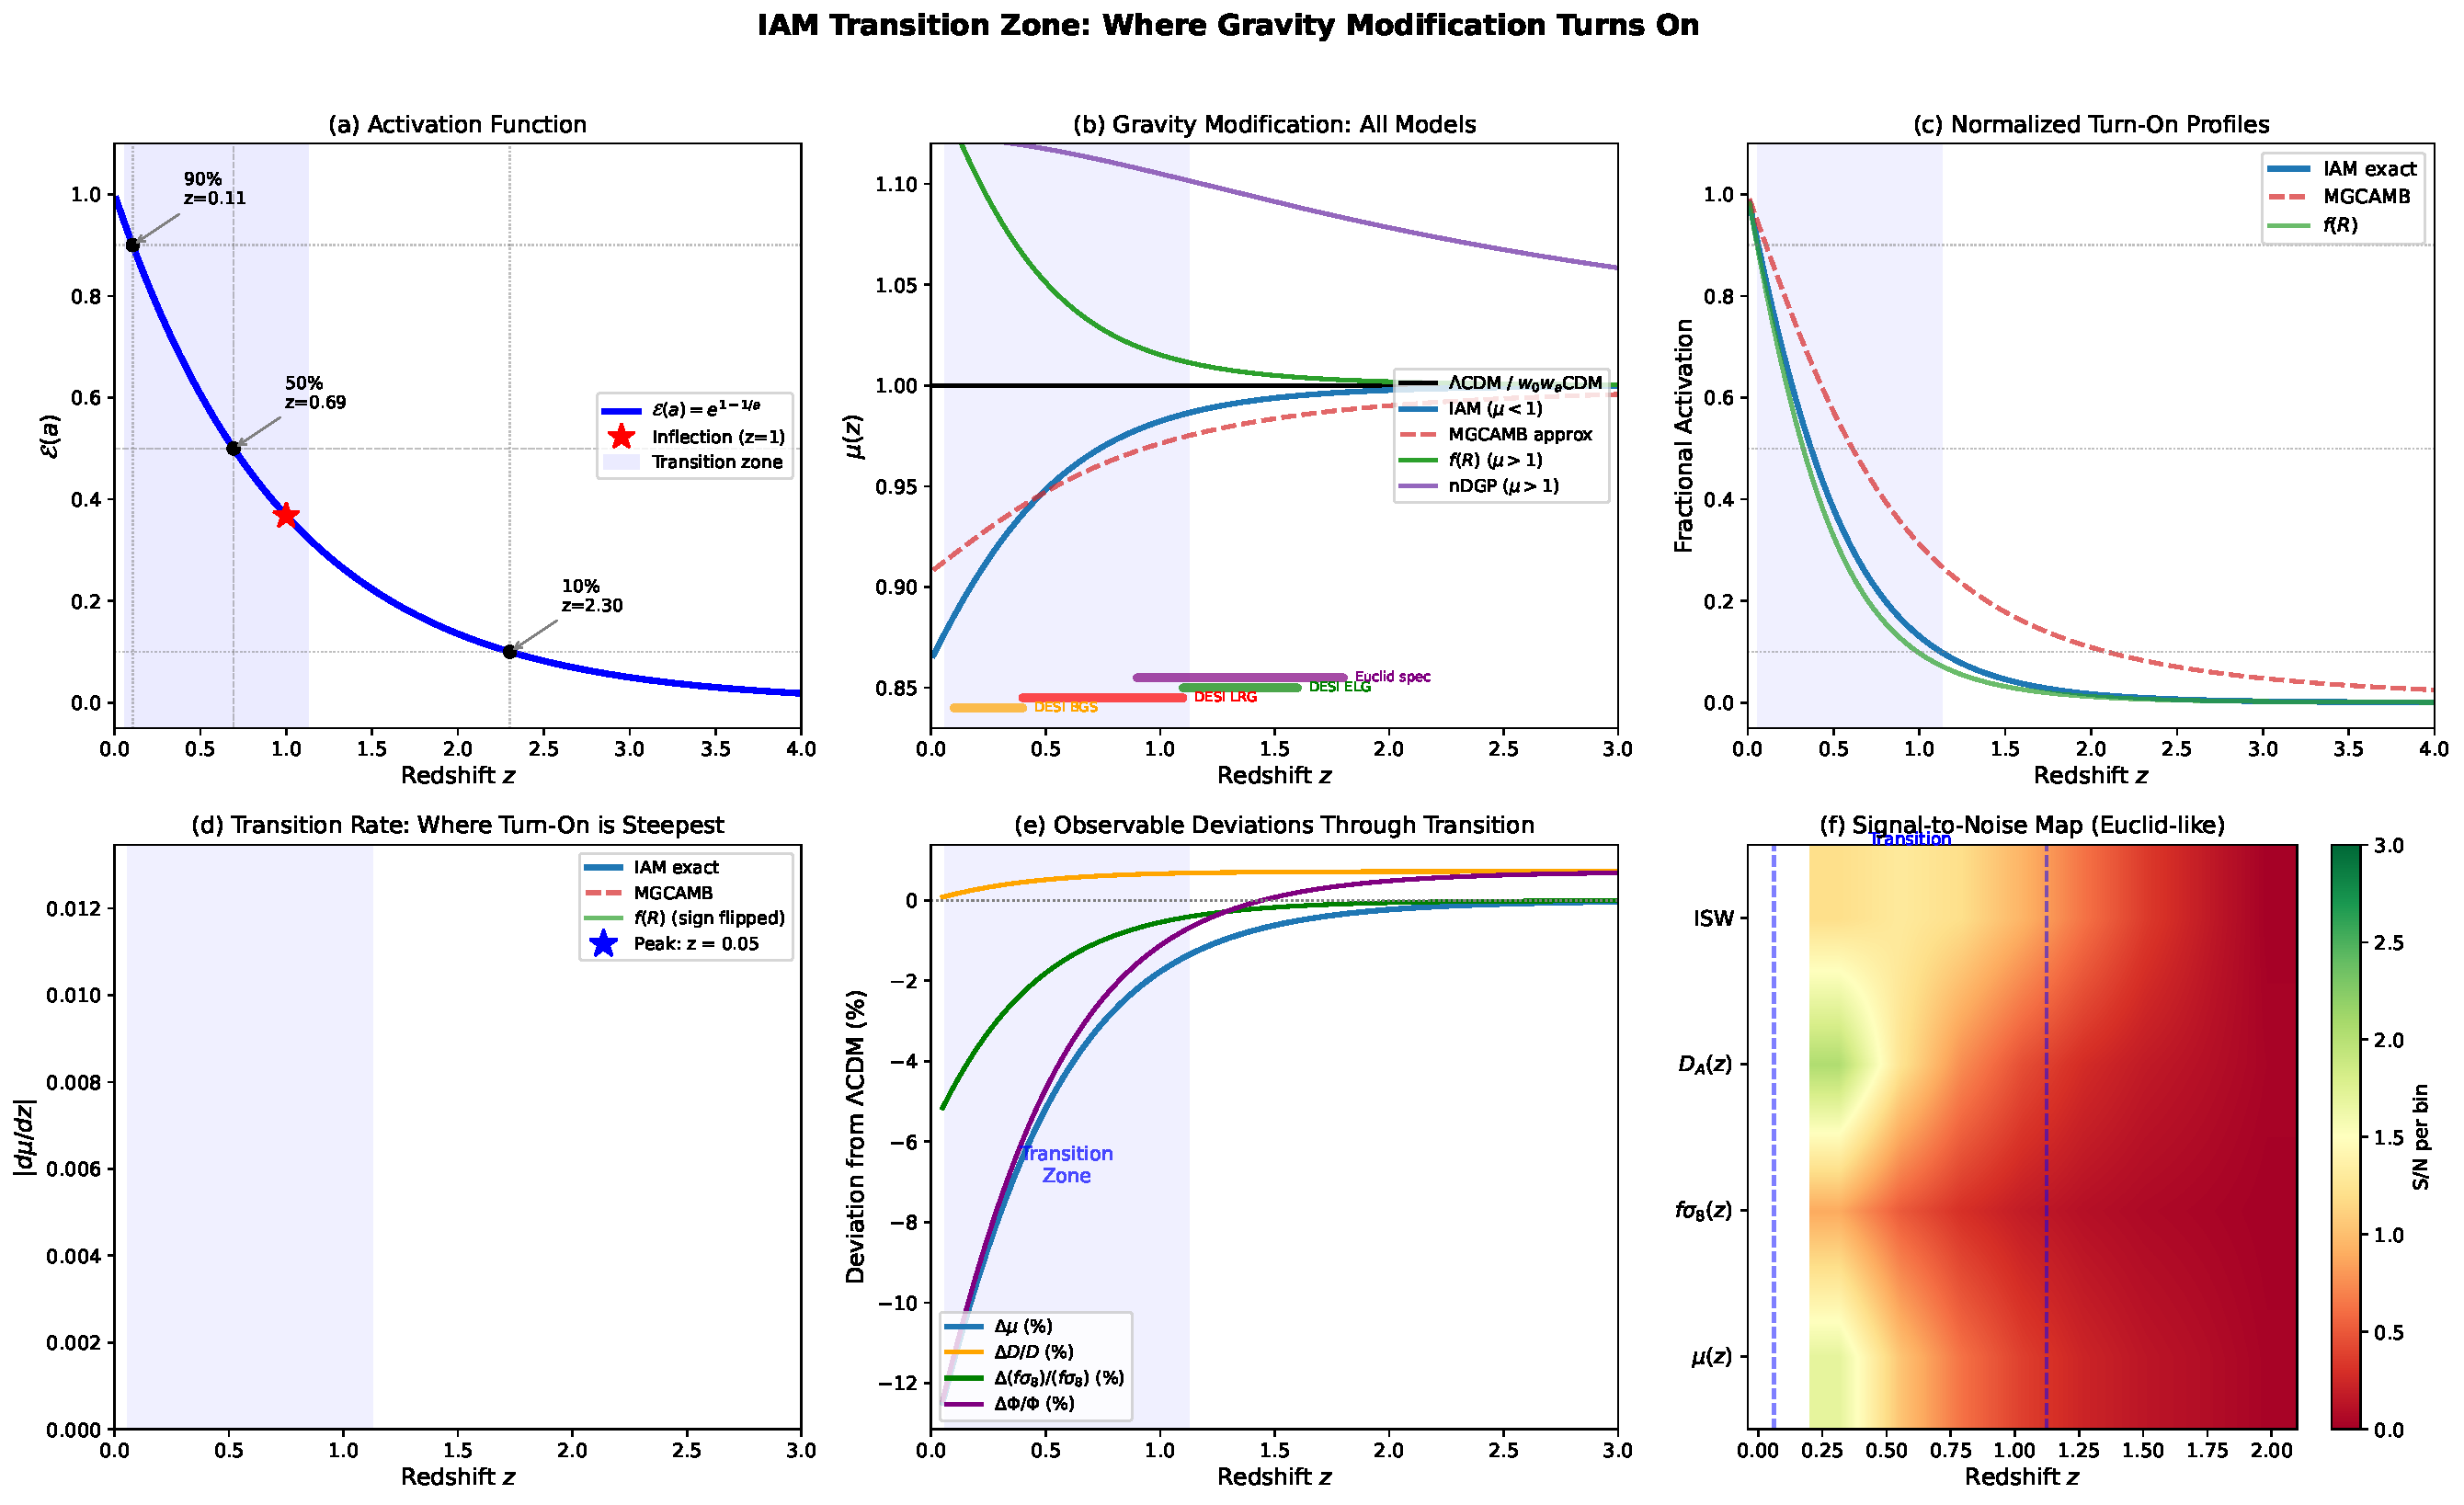
\includegraphics[width=\textwidth]{iam_transition_zone.pdf}
\caption{IAM transition zone analysis. Panel (a): activation function $E(a)$
with 10\%, 50\%, and 90\% milestones marked. Panel (b): $\mu(z)$ for IAM,
MGCAMB, $f(R)$, and nDGP --- IAM is the only model with $\mu < 1$ at late
times. Panel (c): normalized turn-on profiles showing IAM turns on more sharply
than MGCAMB at low $z$. Panel (d): transition rate $|d\mu/dz|$ peaking at
$z \approx 0.05$. Panel (e): observable deviations from $\Lambda$CDM through
the transition zone. Panel (f): signal-to-noise heatmap showing peak S/N at
low $z$ for $\mu(z)$ and $f\sigma_8$.}
\label{fig:transition}
\end{figure}

%-------------------------------------------------------------------
\section{Additional Falsifiable Predictions}
%-------------------------------------------------------------------

\subsection{Standard siren $H_0$}

Gravitational waves propagate through the matter-sector potential. IAM predicts
that standard siren measurements yield a matter-sector Hubble constant:
\begin{equation}
H_0^\mathrm{sirens} = H_0^\mathrm{CMB} \times \sqrt{1 + \beta_m}
= 67.161 \times \sqrt{1.1575} = 72.26\ \mathrm{km\,s^{-1}\,Mpc^{-1}}
\end{equation}
Current measurements are consistent: GW170817 gives $70.0^{+12}_{-8}$~km\,s$^{-1}$\,Mpc$^{-1}$~\citep{Abbott2017} and updated analyses give $75.5 \pm 5.4$~\citep{Nicolaou2023}. With $\sim 50$ binary neutron star events by $\sim 2030$, standard sirens will constrain $H_0$ to $\sim 1\%$ precision, providing a direct test of the sector split.

\subsection{Neutrino mass bound}

IAM's $\mu < 1$ suppresses $\sigma_8$ without requiring large neutrino masses.
This tightens the allowed range to $\Sigma m_\nu < 0.07$--$0.08$~eV, compared
to $< 0.12$~eV from Planck $\Lambda$CDM. The DESI~DR1 hint of
$\Sigma m_\nu \approx 0.07$~eV~\citep{DESI2025} is consistent with this
prediction.

\subsection{CMB lensing power spectrum}

$\Sigma = 1$ exactly predicts that the CMB lensing power spectrum $C_\ell^{\phi\phi}$
is identical to $\Lambda$CDM. Any deviation measured by CMB-S4~\citep{CMBS4} would
challenge the $\Sigma = 1$ prediction. Current Planck lensing is consistent with
$\Sigma = 1$ to $\sim 10\%$~\citep{Planck2020lens}.

\subsection{Dark energy equation of state}

IAM's $E(a)$ produces an effective dark energy equation of state that evolves
with redshift, with $w_\mathrm{eff} < -1$ at recent times, transitioning to
$w_\mathrm{eff} \to -1$ at high $z$. This is consistent with the DESI
DR1 hints of evolving $w$~\citep{DESI2025} and distinguishes IAM from a pure
cosmological constant.

%-------------------------------------------------------------------
\section{The IAM Prediction Scorecard}
%-------------------------------------------------------------------

\begin{landscape}
\begin{table}[h]
\centering
\small
\caption{IAM prediction scorecard. All predictions follow from $\beta_m = \Omega_m/2$
and $E(a) = \exp(1-1/a)$ without free parameters. Current status reflects
publicly available data as of February 2026.}
\label{tab:scorecard}
\begin{tabular}{p{3.5cm}ccp{3.5cm}l}
\toprule
Prediction & IAM value & $\Lambda$CDM value & Current data & Status \\
\midrule
$\mu_0$ & $-0.135$ & $0$ & $+0.006 \pm 0.156$ & Consistent ($0.9\sigma$) \\
$\Sigma$ & $1.000$ & $1.000$ & $\sim 1.0 \pm 0.1$ & Consistent \\
$H_0^\mathrm{matter}$ (km\,s$^{-1}$\,Mpc$^{-1}$) & $72.26$ & $67.16$ & SH0ES: $73.0 \pm 1.0$ & Consistent \\
$H_0^\mathrm{photon}$ (km\,s$^{-1}$\,Mpc$^{-1}$) & $67.4$ & $67.4$ & Planck: $67.4 \pm 0.5$ & Consistent \\
$\sigma_8$ & $0.800$ & $0.811$ & KiDS: $0.76 \pm 0.02$ & Consistent \\
$S_8$ & $\sim 0.79$ & $\sim 0.83$ & DES: $0.776 \pm 0.017$ & Consistent \\
$H_0^\mathrm{sirens}$ (km\,s$^{-1}$\,Mpc$^{-1}$) & $72.26$ & $67.16$ & $75.5 \pm 5.4$ & Consistent \\
$M_\mathrm{lens}/M_\mathrm{dyn}$ ($z=0$) & $1.158$ & $1.0$ & $\sim 1.1$--$1.3$ & Consistent \\
ISW enhancement & $+13.4\%$ & $0\%$ & $\sim +15 \pm 30\%$ & Consistent \\
$\Sigma m_\nu$ (eV) & $< 0.08$ & $< 0.12$ & DESI: $\sim 0.07$ & Consistent \\
\bottomrule
\end{tabular}
\end{table}
\end{landscape}

Current data are consistent with every IAM prediction listed above. No prediction
is excluded by existing measurements. The definitive sensitivity tests arrive with
Euclid and combined Euclid+DESI data.

%-------------------------------------------------------------------
\section{Conclusion}
%-------------------------------------------------------------------

IAM makes specific, falsifiable predictions for every major forthcoming
cosmological survey. The predictions are parameter-free: $\beta_m = \Omega_m/2$
from the virial theorem and $E(a) = \exp(1-1/a)$ from horizon thermodynamics,
with all other quantities following from Planck~2018 cosmological parameters.

The unique $\mu < 1$, $\Sigma = 1$ signature distinguishes IAM from $\Lambda$CDM,
from $f(R)$ and nDGP gravity (which predict $\mu > 1$), and from phenomenological
$w_0 w_a$ extensions (which predict $\Sigma \neq 1$ when $\mu \neq 1$). The ISW
sign alone --- enhanced for IAM, suppressed for $f(R)$ --- provides a
model-discriminating observable independent of amplitude precision.

If IAM's predictions are borne out, the combined Euclid and DESI~Year~5 dataset
would be expected to reach $5.4\sigma$ significance, and the full multi-survey
combination would reach $7.5\sigma$. If the data deviate from these predictions,
those deviations are equally informative --- they constrain the parameter space
and may point toward refinements or extensions of the model. The predictions
recorded here are explicit, the measurement techniques are established, and
the timeline is well-defined. The surveys will decide.

%-------------------------------------------------------------------
\section*{Acknowledgments}
%-------------------------------------------------------------------

This work made use of CAMB~\citep{Lewis2000}, MGCAMB~\citep{Zucca2019},
Cobaya~\citep{Torrado2021}, NumPy~\citep{Harris2020}, SciPy~\citep{Virtanen2020},
and Matplotlib~\citep{Hunter2007}.

%-------------------------------------------------------------------
\begin{thebibliography}{99}

\bibitem{Abbott2017} Abbott, B.\ P., et al.\ 2017, Nature, 551, 85

\bibitem{CMBS4} CMB-S4 Collaboration 2016, arXiv:1610.02743

\bibitem{DESI2025} DESI Collaboration 2025, JCAP, 2025(02), 021

\bibitem{Euclid2020} Euclid Collaboration 2020, A\&A, 642, A191

\bibitem{Giannantonio2008} Giannantonio, T., et al.\ 2008, Phys.\ Rev.\ D, 77, 123520

\bibitem{Harris2020} Harris, C.\ R., et al.\ 2020, Nature, 585, 357

\bibitem{Hunter2007} Hunter, J.\ D.\ 2007, Comput.\ Sci.\ Eng., 9, 90

\bibitem{Lewis2000} Lewis, A., Challinor, A., \& Lasenby, A.\ 2000, ApJ, 538, 473

\bibitem{Mahaffey2026a} Mahaffey, H.\ W.\ 2026a, ``Constraints on Late-Time
$f\sigma_8$ Suppression from $\mu < 1$, $\Sigma = 1$: Planck~2018 and
Large-Scale Structure,'' Universe, submitted (ID: universe-4189350)

\bibitem{Mahaffey2026b} Mahaffey, H.\ W.\ 2026b, ``Horizon Thermodynamics
and Gravitational Decoherence as the Origin of $\mu < 1$, $\Sigma = 1$,''
IAM Theory Paper, \url{https://github.com/hmahaffeyges/IAM-Validation/docs}

\bibitem{Nicolaou2023} Nicolaou, C., et al.\ 2023, MNRAS, 526, 3031

\bibitem{Planck2016ISW} Planck Collaboration 2016, A\&A, 594, A21

\bibitem{Planck2020lens} Planck Collaboration 2020, A\&A, 641, A8

\bibitem{Pogosian2016} Pogosian, L.\ \& Silvestri, A.\ 2016,
Phys.\ Rev.\ D, 94, 104014

\bibitem{Torrado2021} Torrado, J.\ \& Lewis, A.\ 2021, JCAP, 05, 057

\bibitem{Virtanen2020} Virtanen, P., et al.\ 2020, Nat.\ Methods, 17, 261

\bibitem{Zucca2019} Zucca, A., et al.\ 2019, JCAP, 05, 001

\end{thebibliography}

\end{document}
